\documentclass[border=4pt,12pt]{standalone}
% House style for redrawn exam diagrams (diagram-v4: 0.4pt lines, filled -latex arrows, fine dashes; stipple and hatching drawn as real dots/lines (no PDF/SVG patterns, so they render in every browser and at any scale); transparent background). Every figure \input's this.
\usepackage{amsmath,amssymb}
\usepackage{txfonts}
\usepackage{pdfrender,xcolor}
% \halo{text}: label on shading. The shading stops just around each letter's outline (a thin knock-out that follows the
% glyphs, like the papers' typesetting), never a box. Owner: "I don't want a box around the text".
\newcommand{\halo}[1]{\leavevmode\rlap{\pdfrender{TextRenderingMode=2,LineWidth=2.2pt,LineJoinStyle=1,StrokeColor=white,FillColor=white}#1}#1}
\usepackage{tikz,pgfplots}
\pgfplotsset{compat=1.18}
\usetikzlibrary{arrows.meta,calc,angles,quotes,patterns,patterns.meta,intersections,positioning,decorations.markings,shapes.geometric}
% Stipple and hatching are drawn as actual dots / lines clipped to the region (path picture), NOT as pattern fills:
% SVG <pattern> fills vanish or blur when browsers scale the image, so the owner could not see the shading.
% Each dot is a 0.72pt square (keeps SVGs small; reads as a dot at print size). Dots sit on one global staggered grid, so neighbouring regions line up.
\makeatletter
\newdimen\ex@x \newdimen\ex@y \newdimen\ex@xa \newdimen\ex@ya \newdimen\ex@xb \newdimen\ex@yb \newcount\ex@row
\def\exam@stipplecolor{black!75}\def\exam@dotr{0.42pt}\def\exam@dotgap{2.5}
\def\ex@rowdots{\ifdim\ex@x<\ex@xb \pgfpathrectangle{\pgfqpoint{\dimexpr\ex@x-0.36pt\relax}{\dimexpr\ex@y-0.36pt\relax}}{\pgfqpoint{0.72pt}{0.72pt}}\advance\ex@x by \exam@dotgap pt\relax\expandafter\ex@rowdots\fi}
\def\exam@stipple{%
  \pgftransformreset% dots are sized in real points even inside scaled pictures
  \pgfpointanchor{path picture bounding box}{south west}\ex@xa=\pgf@x \ex@ya=\pgf@y
  \pgfpointanchor{path picture bounding box}{north east}\ex@xb=\pgf@x \ex@yb=\pgf@y
  \pgfsetfillcolor{\exam@stipplecolor}\pgfmathsetmacro\ex@h{\exam@dotgap/2}%
  \pgfmathtruncatemacro\ex@r{floor(\ex@ya/\ex@h)-1}\ex@row=\ex@r\relax
  \ex@y=\ex@r\dimexpr\ex@h pt\relax
  \loop\ifdim\ex@y<\ex@yb
    \pgfmathtruncatemacro\ex@c{floor(\ex@xa/\exam@dotgap)-1}\ex@x=\ex@c\dimexpr\exam@dotgap pt\relax
    \ifodd\ex@row \advance\ex@x by \ex@h pt\fi
    \ex@rowdots
    \advance\ex@y by \ex@h pt \advance\ex@row by 1
    \ifnum\numexpr\ex@row-(\ex@row/4)*4\relax=0 \pgfusepath{fill}\fi% flush every 4 rows: bounded TeX memory, few clip copies in the SVG
  \repeat\pgfusepath{fill}}
\newdimen\ex@d
\def\exam@hatch#1{% #1 = 1 for /, -1 for \ ; lines 45 degrees, 3pt apart
  \pgftransformreset
  \pgfpointanchor{path picture bounding box}{south west}\ex@xa=\pgf@x \ex@ya=\pgf@y
  \pgfpointanchor{path picture bounding box}{north east}\ex@xb=\pgf@x \ex@yb=\pgf@y
  \ex@d=\dimexpr\ex@yb-\ex@ya\relax \ex@x=\dimexpr\ex@xa-\ex@d\relax
  \loop\ifdim\ex@x<\ex@xb
    \ifnum#1>0 \pgfpathmoveto{\pgfqpoint{\ex@x}{\ex@ya}}\pgfpathlineto{\pgfqpoint{\dimexpr\ex@x+\ex@d\relax}{\ex@yb}}%
    \else \pgfpathmoveto{\pgfqpoint{\ex@x}{\ex@yb}}\pgfpathlineto{\pgfqpoint{\dimexpr\ex@x+\ex@d\relax}{\ex@ya}}\fi
    \advance\ex@x by 4.24pt
  \repeat
  \pgfsetlinewidth{0.4pt}\pgfsetstrokecolor{black}\pgfusepath{stroke}}
\def\examstipple{\exam@stipple}\def\examhatch{\exam@hatch}\def\examsetstipplecolor#1{\def\exam@stipplecolor{#1}}\def\examsetdotgap#1{\def\exam@dotgap{#1}}
\makeatother
% (legacy pattern kept for old files)
% staggered stipple like the NESA papers' dotted shading
\pgfdeclarepatternformonly{exam stipple}{\pgfpointorigin}{\pgfqpoint{2.2pt}{2.2pt}}{\pgfqpoint{2.2pt}{2.2pt}}{%
  \pgfpathcircle{\pgfqpoint{0.55pt}{0.55pt}}{0.42pt}\pgfpathcircle{\pgfqpoint{1.65pt}{1.65pt}}{0.42pt}\pgfusepath{fill}}
\tikzset{
  every picture/.style={line width=0.6pt, >={Latex[length=2mm,width=1.3mm]}},
  curve/.style={line width=0.6pt},
  open arrow/.style={-{Latex[length=2mm,width=1.3mm]}},  % owner: filled -latex heads everywhere, no open chevrons
  aux/.style={dash pattern=on 2pt off 1.5pt, line width=0.6pt},
  shade/.code={\def\exA{#1}\def\exB{none}\ifx\exA\exB\else\pgfkeysalso{fill=black!18}\fi},
  shade/.default=on,
  shade dots/.style={fill=none, path picture={\examstipple}},
  stipple color/.code={\examsetstipplecolor{#1}},
  stipple gap/.code={\examsetdotgap{#1}},
  shade dense dots/.style={fill=none, stipple gap=1.6, path picture={\examstipple}},
  shade hatch/.style={fill=none, path picture={\examhatch{1}}},
  shade hatch reverse/.style={fill=none, path picture={\examhatch{-1}}},
  shade solid/.style={fill=black},
  pt/.style={circle, fill, inner sep=1.1pt},
  open pt/.style={circle, draw, fill=white, inner sep=1.1pt},
}
\pgfplotsset{
  exam axes/.style={axis lines=middle, axis line style={->}, xlabel={$x$}, ylabel={$y$},
    xlabel style={anchor=west}, ylabel style={anchor=south}, tick label style={font=\small},
    every axis plot/.append style={line width=0.6pt, black}, samples=200, clip=false,
    enlargelimits=false, axis on top},
}

\begin{document}
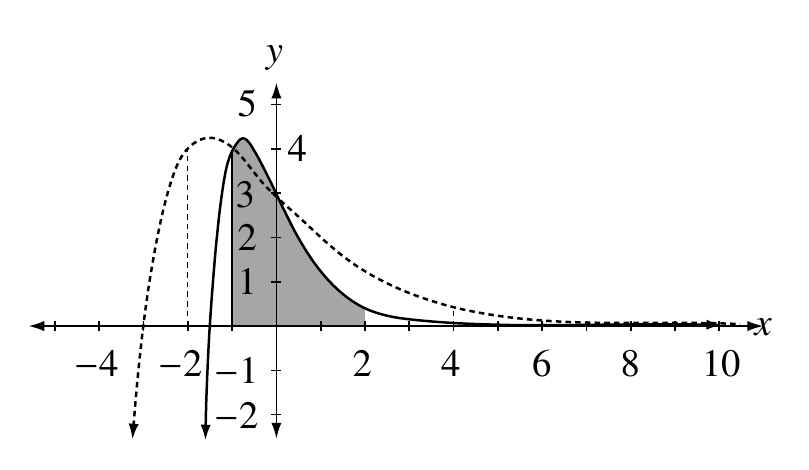
\begin{tikzpicture}[x=0.0127cm,y=-0.0127cm, every node/.style={font=\fontsize{14}{16}\selectfont}]
  % shaded: area under y = f(2x) from x = -1 to x = 2
  \begin{scope}\clip (221.7,0) rectangle (354.6,298.5);
  \fill[black!35] plot[smooth] coordinates {(195,413) (195.3,395.6) (195.7,378.2) (196.3,361) (197,343.5) (197.8,326.3) (198.7,308.9) (199.8,291.5) (201,274.3) (202.3,256.9) (203.7,239.6) (205.2,222.2) (206.9,205.2) (208.7,188.1) (210.8,171.4) (213.2,154.9) (215.9,140.5) (219.3,129) (223.9,119.4) (228.4,113.1) (231.1,111.1) (232.5,110.7) (234,110.9) (236.1,112.1) (240,116.8) (247.2,128.9) (254.7,143.2) (262.1,158.2) (269.5,173.9) (277,189.2) (284.4,203.8) (292.2,217.5) (300.3,230.2) (309,242.1) (318.3,253) (328.2,262.8) (338.6,271.2) (349.1,277.9) (360.1,283.1) (372.5,287.1) (386,290) (401.2,292) (417.8,293.6) (434.6,294.9) (451.6,295.9) (468.6,296.6) (485.9,297.1) (503.1,297.5) (520.3,297.6) (537.7,297.6) (555.1,297.6) (572.7,297.4) (590.1,297.2) (607.7,297) (625.4,296.8) (642.8,296.7) (660.2,296.7) (677.5,296.8) (694.7,297.1) (712,297.6)} -- cycle;
  \end{scope}
  \draw (221.7,298.5) -- (221.7,124);
  \draw[aux] (177,298.5) -- (177,120); \draw[aux] (443,298.5) -- (443,278.5);
  \draw (44.5,293.5) -- (44.5,303.5);
  \draw (88.8,293.5) -- (88.8,303.5);
  \draw (133.1,293.5) -- (133.1,303.5);
  \draw (177.4,293.5) -- (177.4,303.5);
  \draw (221.7,293.5) -- (221.7,303.5);
  \draw (310.3,293.5) -- (310.3,303.5);
  \draw (354.6,293.5) -- (354.6,303.5);
  \draw (398.9,293.5) -- (398.9,303.5);
  \draw (443.2,293.5) -- (443.2,303.5);
  \draw (487.5,293.5) -- (487.5,303.5);
  \draw (531.8,293.5) -- (531.8,303.5);
  \draw (576.1,293.5) -- (576.1,303.5);
  \draw (620.4,293.5) -- (620.4,303.5);
  \draw (664.7,293.5) -- (664.7,303.5);
  \draw (709.0,293.5) -- (709.0,303.5);
  \draw (261,387.1) -- (271,387.1);
  \draw (261,342.8) -- (271,342.8);
  \draw (261,254.2) -- (271,254.2);
  \draw (261,209.9) -- (271,209.9);
  \draw (261,165.6) -- (271,165.6);
  \draw (261,121.3) -- (271,121.3);
  \draw (261,77.0) -- (271,77.0);
  \draw[<->] (18,298.5) -- (753,298.5);
  \draw[<->] (266,411) -- (266,55);
  \draw[curve, aux, line width=0.9pt, <-] plot[smooth] coordinates {(122,412) (123.4,393.8) (124.9,375.8) (126.5,357.8) (128.2,340) (130.1,322.2) (132.1,304.4) (134.3,286.9) (136.7,269.4) (139.4,251.7) (142.3,234.4) (145.4,217.4) (148.8,200.2) (152.5,183.5) (156.7,167.3) (161.3,151.9) (166.1,138.9) (171.1,129.1) (176.8,121.5) (183.1,115.9) (189.5,112.2) (195.8,110.4) (201.4,110.2) (207.9,111.7) (215.5,115.3) (223.3,121.1) (231.5,129.5) (241.1,141.5) (250.8,153.6) (260.6,164.1) (272.4,175.1) (285.4,186.6) (298.3,198.5) (311.3,210.6) (323.7,221.4) (335.8,231) (348.4,239.8) (361.5,247.7) (375.3,255) (389.5,261.6) (404.4,267.6) (419.6,272.8) (435.1,277.5) (451,281.5) (467.1,284.8) (483.5,287.6) (500.2,289.9) (517,291.7) (534.1,293.1) (551.3,294.1) (568.7,294.8) (586.5,295.2) (604.2,295.4) (622.4,295.4) (640.6,295.4) (658.8,295.3) (676.9,295.4) (694.7,295.5) (712.4,295.9) (730,296.5)};
  \draw[curve, line width=0.9pt, <->] plot[smooth] coordinates {(195,413) (195.3,395.6) (195.7,378.2) (196.3,361) (197,343.5) (197.8,326.3) (198.7,308.9) (199.8,291.5) (201,274.3) (202.3,256.9) (203.7,239.6) (205.2,222.2) (206.9,205.2) (208.7,188.1) (210.8,171.4) (213.2,154.9) (215.9,140.5) (219.3,129) (223.9,119.4) (228.4,113.1) (231.1,111.1) (232.5,110.7) (234,110.9) (236.1,112.1) (240,116.8) (247.2,128.9) (254.7,143.2) (262.1,158.2) (269.5,173.9) (277,189.2) (284.4,203.8) (292.2,217.5) (300.3,230.2) (309,242.1) (318.3,253) (328.2,262.8) (338.6,271.2) (349.1,277.9) (360.1,283.1) (372.5,287.1) (386,290) (401.2,292) (417.8,293.6) (434.6,294.9) (451.6,295.9) (468.6,296.6) (485.9,297.1) (503.1,297.5) (520.3,297.6) (537.7,297.6) (555.1,297.6) (572.7,297.4) (590.1,297.2) (607.7,297) (625.4,296.8) (642.8,296.7) (660.2,296.7) (677.5,296.8) (694.7,297.1) (712,297.6)};
  \node at (264,30) {$y$};
  \node at (752,300) {$x$};
  \node at (86,336) {$-4$};
  \node at (170,336) {$-2$};
  \node at (352,336) {$2$};
  \node at (440.5,336) {$4$};
  \node at (531.5,336) {$6$};
  \node at (620,336) {$8$};
  \node at (711,336) {$10$};
  \node at (237,76) {$5$};
  \node at (287,121) {$4$};
  \node at (235,167) {$3$};
  \node at (237,210) {$2$};
  \node at (237,254) {$1$};
  \node at (226,343) {$-1$};
  \node at (226,388) {$-2$};
\end{tikzpicture}
\end{document}
